\documentclass{beamer}
\usetheme{metropolis}

\usepackage[spanish]{babel}
\usepackage[utf8]{inputenc}
\usepackage{graphicx}
\usepackage{tikz}
\usepackage{xcolor}
\usepackage{amsmath}
\usepackage{listings}
\usepackage{fontawesome}
\usepackage{booktabs}

\usetikzlibrary{positioning,shapes.multipart,calc,arrows,shapes.geometric}

% Definición de colores personalizados
\definecolor{primary}{RGB}{46, 204, 113}
\definecolor{secondary}{RGB}{52, 152, 219}
\definecolor{accent}{RGB}{231, 76, 60}
\definecolor{background}{RGB}{236, 240, 241}
\definecolor{gradient1}{RGB}{255, 107, 107}
\definecolor{gradient2}{RGB}{255, 159, 67}

% Configuración del tema
\setbeamercolor{normal text}{fg=black,bg=background}
\setbeamercolor{structure}{fg=primary}
\setbeamercolor{alerted text}{fg=accent}

\definecolor{lightgray}{rgb}{0.95,0.95,0.95}
\definecolor{darkgreen}{rgb}{0,0.5,0}
\definecolor{darkblue}{rgb}{0,0,0.5}

\lstset{
  backgroundcolor=\color{lightgray},
  basicstyle=\tiny\ttfamily,
  keywordstyle=\color{darkblue}\bfseries,
  commentstyle=\color{darkgreen},
  stringstyle=\color{red},
  numbers=left,
  numberstyle=\tiny\color{gray},
  stepnumber=1,
  numbersep=5pt,
  showspaces=false,
  showstringspaces=false,
  showtabs=false,
  frame=single,
  tabsize=2,
  language=Python,
  breaklines=true,
  breakatwhitespace=true
}

\title{\Huge\textbf{NoSQL}}
\author{Gestión y Arquitectura de Datos}
\date{}

\begin{document}

\begin{frame}
    \titlepage
    \begin{tikzpicture}[remember picture,overlay]
        \node[anchor=south west,inner sep=30pt] at (current page.south west) {
            
\includegraphics[height=1cm]{../misc/UdeSA.png}
        };
    \end{tikzpicture}
\end{frame}

\begin{frame}{¿Por qué surge NoSQL?}
    Las bases de datos NoSQL surgieron como respuesta a limitaciones específicas de las bases de datos relacionales:
    
    \begin{itemize}
        \item \textbf{Escalabilidad}: Escalado horizontal vs vertical
        \item \textbf{Flexibilidad}: Esquemas rígidos vs flexibles
        \item \textbf{Big Data}: Manejo de datos no estructurados
        \item \textbf{Velocidad}: Alta velocidad en lectura/escritura
        \item \textbf{Disponibilidad}: Sistemas distribuidos
    \end{itemize}
\end{frame}

\begin{frame}{Tipos de Bases de Datos NoSQL}
    \begin{center}
        \begin{tabular}{cccc}
            \begin{minipage}{2.2cm}
                \centering
                {\Large \faFileText}\\[0.2cm]
                \textbf{Documentales}\\[0.1cm]
            \end{minipage} &
            \begin{minipage}{2.2cm}
                \centering
                {\Large \faKey}\\[0.2cm]
                \textbf{Clave-Valor}\\[0.1cm]
            \end{minipage} &
            \begin{minipage}{2.2cm}
                \centering
                {\Large \faTable}\\[0.2cm]
                \textbf{Columnares}\\[0.1cm]
            \end{minipage} &
            \begin{minipage}{2.2cm}
                \centering
                {\Large \faShare}\\[0.2cm]
                \textbf{De Grafos}\\[0.1cm]
            \end{minipage}
        \end{tabular}
    \end{center}
\end{frame}

\begin{frame}{Bases de Datos Documentales}
    \begin{columns}
        \begin{column}{0.6\textwidth}
            \textbf{Características:}
            \begin{itemize}
                \item Almacenan datos en documentos JSON
                \item Flexibilidad en esquemas
                \item Datos anidados y no estructurados
                \item Fáciles de usar
            \end{itemize}
        \end{column}
        \begin{column}{0.4\textwidth}
            \centering
            
\includegraphics[width=0.8\textwidth]{images/Mongodb.png}
        \end{column}
    \end{columns}
\end{frame}

\begin{frame}[fragile]{Ejemplo de Base de Datos Documental}
    \begin{lstlisting}
{
  "id": "1",
  "cliente": {
    "nombre": "Juan Garcia",
    "email": ["juan@email.com", "juan.g@email.com"],
    "direcciones": [
      {
        "tipo": "casa",
        "calle": "Av. Libertador 1234"
      }
    ]
  },
  "pedidos": [
    {
      "fecha": "2024-01-01",
      "total": 1500
    }
  ]
}
    \end{lstlisting}
\end{frame}

\begin{frame}{Bases de Datos Clave-Valor}
    \begin{columns}
        \begin{column}{0.6\textwidth}
            \textbf{Características:}
            \begin{itemize}
                \item Almacenan pares clave-valor
                \item Alta velocidad
                \item Simplicidad
                \item Ideales para cachés
            \end{itemize}
        \end{column}
        \begin{column}{0.4\textwidth}
            \centering
            
\includegraphics[width=0.8\textwidth]{images/Redis.png}
        \end{column}
    \end{columns}
\end{frame}

\begin{frame}[fragile]{Ejemplo de Base de Datos Clave-Valor}
    \begin{lstlisting}
SET usuario:1 "Juan Garcia"
SET usuario:1:email "juan@email.com"
SET carrito:1 "['producto1', 'producto2']"
    \end{lstlisting}
\end{frame}

\begin{frame}{Bases de Datos Columnares}
    \begin{columns}
        \begin{column}{0.6\textwidth}
            \textbf{Características:}
            \begin{itemize}
                \item Almacenan datos en columnas
                \item Eficiencia en análisis
                \item Escalabilidad horizontal
                \item Mejor compresión
            \end{itemize}
        \end{column}
        \begin{column}{0.4\textwidth}
            \centering
            
\includegraphics[width=0.8\textwidth]{images/Cassandra.png}
        \end{column}
    \end{columns}
\end{frame}

\begin{frame}{Bases de Datos de Grafos}
    \begin{columns}
        \begin{column}{0.6\textwidth}
            \textbf{Características:}
            \begin{itemize}
                \item Representan relaciones entre entidades
                \item Consultas eficientes de relaciones
                \item Ideales para redes sociales
                \item Sistemas de recomendación
            \end{itemize}
        \end{column}
        \begin{column}{0.4\textwidth}
            \centering
            
\includegraphics[width=0.8\textwidth]{images/Neo4j.png}
        \end{column}
    \end{columns}
\end{frame}

\begin{frame}{Ejemplo de Grafo}
    \begin{center}
        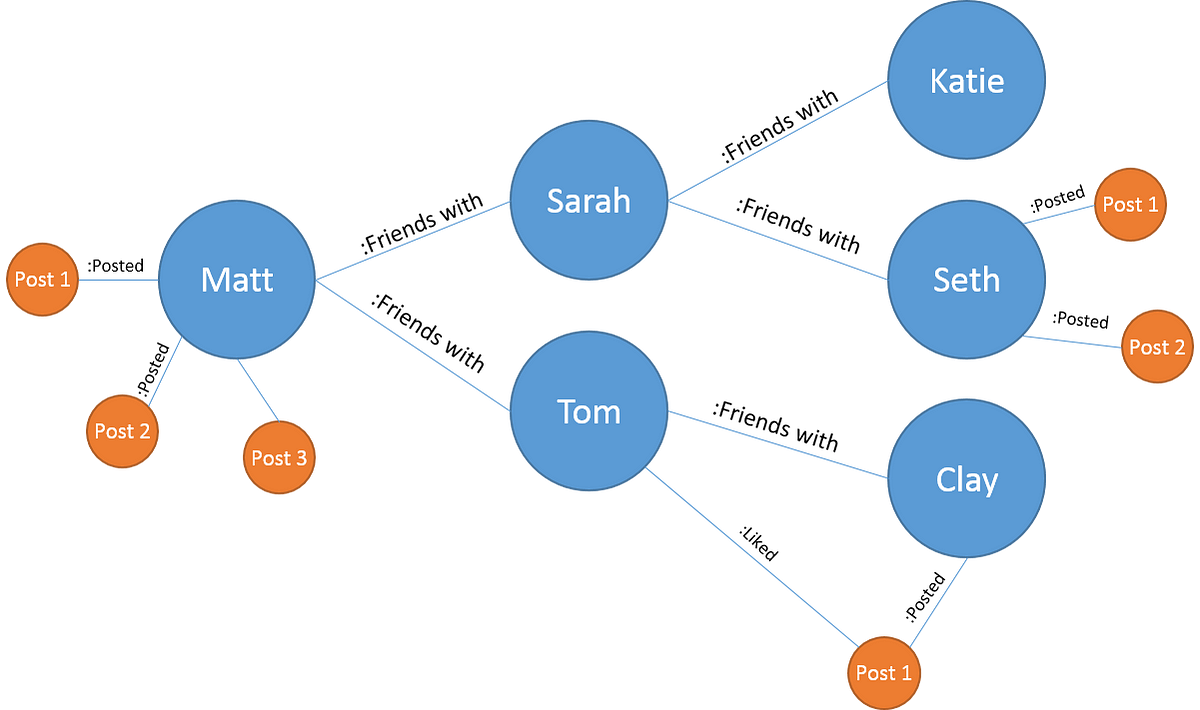
\includegraphics[width=0.7\textwidth]{images/Neo4j_graph.png}
    \end{center}
\end{frame}

\begin{frame}{Teorema CAP}
    Un sistema distribuido no puede garantizar simultáneamente:
    
    \begin{center}
        \begin{tabular}{ccc}
            \begin{minipage}{2.5cm}
                \centering
                {\Large \faCheckCircle}\\[0.2cm]
                \textbf{Consistency}\\[0.1cm]
                {\scriptsize Todos ven los mismos datos}
            \end{minipage} &
            \begin{minipage}{2.5cm}
                \centering
                {\Large \faClockO}\\[0.2cm]
                \textbf{Availability}\\[0.1cm]
                {\scriptsize Cada petición recibe respuesta}
            \end{minipage} &
            \begin{minipage}{3.3cm}
                \centering
                {\Large \faShield}\\[0.2cm]
                \textbf{Partition Tolerance}\\[0.1cm]
                {\scriptsize Funciona aún con fallos de red}
            \end{minipage}
        \end{tabular}
    \end{center}
\end{frame}

\begin{frame}{Clasificación CAP de Bases de Datos}
    \begin{center}
        \begin{tabular}{lll}
        \toprule
        Base de Datos & Prioriza & Sacrifica \\
        \midrule
        MongoDB & CP & Availability \\
        Cassandra & AP & Consistency \\
        Redis & CP & Availability \\
        Neo4j & CA & Partition Tolerance \\
        \bottomrule
        \end{tabular}
    \end{center}
    
    \vspace{0.5cm}
    \textbf{Nota}: MongoDB es configurable para priorizar Consistency o Availability.
\end{frame}

\begin{frame}{Cuándo Usar NoSQL}
    \textbf{Casos de uso ideales:}
    \begin{itemize}
        \item \textbf{Datos no estructurados}: Sin esquema fijo
        \item \textbf{Escalabilidad horizontal}: Añadir servidores
        \item \textbf{Alta velocidad}: Lectura/escritura rápidas
        \item \textbf{Agilidad}: Desarrollo rápido
        \item \textbf{Big Data}: Grandes volúmenes de datos
    \end{itemize}
\end{frame}

\begin{frame}{Cuándo NO Usar NoSQL}
    \textbf{Casos donde evitar NoSQL:}
    \begin{itemize}
        \item \textbf{Datos altamente relacionales}: Muchas relaciones complejas
        \item \textbf{Transacciones ACID}: Garantías estrictas
        \item \textbf{Reportes complejos}: Múltiples JOINs
        \item \textbf{Equipos sin experiencia}: Curva de aprendizaje
    \end{itemize}
\end{frame}

\begin{frame}{Comparación: SQL vs NoSQL}
    \begin{center}
        \begin{tabular}{lcc}
        \toprule
        Característica & SQL & NoSQL \\
        \midrule
        Esquema & Fijo & Flexible \\
        Escalabilidad & Vertical & Horizontal \\
        Transacciones & ACID & Eventual \\
        Consultas & Complejas & Simples \\
        Curva aprendizaje & Baja & Media-Alta \\
        \bottomrule
        \end{tabular}
    \end{center}
\end{frame}

\begin{frame}{Terminamos}
    \begin{center}
        \Large{\textbf{¿Dudas?\\¿Consultas?}}
    \end{center}
    \begin{tikzpicture}[remember picture,overlay]
        \node[anchor=south,inner sep=30pt] at (current page.south) {
            
\includegraphics[height=1cm]{../misc/UdeSA.png}
        };
    \end{tikzpicture}
\end{frame}

\end{document}
